\section{The Matrix-Based Characterization}\label{sec:matrix_approach}

In this section, we develop an alternative, matrix-based characterization of cubic irrationals that provides a deeper theoretical understanding of the \HAPD{} algorithm. While Karpenkov \cite{Karpenkov2022} used matrix representations primarily in the context of Dirichlet groups, we expand this approach by establishing a more explicit connection between cubic irrationals and the properties of companion matrices, offering a complementary perspective on Hermite's problem.

This matrix-based characterization builds upon Karpenkov's insights regarding the relationship between matrices and cubic irrationals, but develops a more comprehensive theoretical framework focused specifically on trace relations and companion matrix properties. Our approach enhances the connection between the algorithmic method and the underlying algebraic structure.

\subsection{Companion Matrices and Minimal Polynomials}

We begin with the necessary definitions and background on companion matrices.

\begin{definition}[Companion Matrix]
For a monic polynomial $p(x) = x^n + a_{n-1}x^{n-1} + \cdots + a_1x + a_0$, the companion matrix $C_p$ is the $n \times n$ matrix:
\begin{equation}
C_p = \begin{pmatrix}
0 & 0 & \cdots & 0 & -a_0 \\
1 & 0 & \cdots & 0 & -a_1 \\
0 & 1 & \cdots & 0 & -a_2 \\
\vdots & \vdots & \ddots & \vdots & \vdots \\
0 & 0 & \cdots & 1 & -a_{n-1}
\end{pmatrix}
\end{equation}
\end{definition}

\begin{proposition}[Properties of Companion Matrices]\label{prop:companion_properties}
Let $p(x) = x^n + a_{n-1}x^{n-1} + \cdots + a_1x + a_0$ be a monic polynomial and $C_p$ its companion matrix. Then:
\begin{enumerate}
    \item The characteristic polynomial of $C_p$ is exactly $p(x)$
    \item The eigenvalues of $C_p$ are precisely the roots of $p(x)$
    \item For any $k \geq 1$, $\tr(C_p^k) = \sum_{i=1}^{n} \lambda_i^k$, where $\lambda_1, \lambda_2, \ldots, \lambda_n$ are the eigenvalues of $C_p$
\end{enumerate}
\end{proposition}

\begin{proof}
These are standard results in linear algebra. For a detailed proof, see \cite{Horn2012}.
\end{proof}

\subsection{Trace Characterization of Cubic Irrationals}

We now develop a characterization of cubic irrationals based on the traces of powers of companion matrices.

\begin{theorem}[Matrix Characterization of Cubic Irrationals]\label{thm:matrix_cubic}
Let $\alpha$ be a real number. Then $\alpha$ is a cubic irrational if and only if there exists a $3 \times 3$ companion matrix $C$ such that:
\begin{enumerate}
    \item The characteristic polynomial of $C$ is irreducible over $\Q$
    \item For any $k \geq 1$, $\tr(C^k) = \alpha^k + \beta^k + \gamma^k$, where $\beta$ and $\gamma$ are the other roots of the minimal polynomial of $\alpha$
\end{enumerate}
\end{theorem}

\begin{proof}
($\Rightarrow$) Suppose $\alpha$ is a cubic irrational with minimal polynomial $f(x) = x^3 + px^2 + qx + r$ where $p, q, r \in \Q$ and the polynomial is irreducible.

Let $C$ be the companion matrix of $f$:
\begin{equation}
C = \begin{pmatrix}
0 & 0 & -r \\
1 & 0 & -q \\
0 & 1 & -p
\end{pmatrix}
\end{equation}

By Proposition \ref{prop:companion_properties}, the characteristic polynomial of $C$ is $f(x) = x^3 + px^2 + qx + r$, which is irreducible over $\Q$ by assumption.

Let $\beta$ and $\gamma$ be the other roots of $f$. The eigenvalues of $C$ are precisely $\alpha, \beta, \gamma$. By Proposition \ref{prop:companion_properties}, for any $k \geq 1$:
\begin{equation}
\tr(C^k) = \alpha^k + \beta^k + \gamma^k
\end{equation}

This establishes the forward direction.

($\Leftarrow$) Conversely, suppose there exists a $3 \times 3$ companion matrix $C$ satisfying the given conditions.

Since the characteristic polynomial of $C$ is irreducible over $\Q$ and has degree 3, it must be the minimal polynomial of all its roots. Let these roots be $\alpha, \beta, \gamma$. By condition 2, we have:
\begin{equation}
\tr(C^k) = \alpha^k + \beta^k + \gamma^k
\end{equation}

This implies that $\alpha$ is an eigenvalue of $C$ and thus a root of the irreducible cubic polynomial $\det(xI - C)$. Therefore, $\alpha$ is a cubic irrational.
\end{proof}

\begin{corollary}[Cubic Irrational Power Sums]\label{cor:power_sums}
If $\alpha$ is a cubic irrational with minimal polynomial $x^3 + px^2 + qx + r$, and $\beta, \gamma$ are the other roots, then the power sums $s_k = \alpha^k + \beta^k + \gamma^k$ satisfy the recurrence relation:
\begin{equation}
s_k = -p \cdot s_{k-1} - q \cdot s_{k-2} - r \cdot s_{k-3} \quad \text{for } k \geq 3
\end{equation}
with initial conditions $s_0 = 3, s_1 = 0, s_2 = -2p$.
\end{corollary}

\begin{proof}
This follows from Newton's identities relating power sums to the coefficients of the minimal polynomial, combined with the trace formula from Theorem \ref{thm:matrix_cubic}.
\end{proof}

\subsection{Connection to Field Extensions and Galois Theory}

The matrix characterization connects naturally to the Galois-theoretic perspective discussed in Section \ref{sec:galois_theory}.

\begin{proposition}[Matrix and Field Extensions]\label{prop:matrix_field}
Let $\alpha$ be a cubic irrational with minimal polynomial $f(x)$ and companion matrix $C$. Then:
\begin{enumerate}
    \item The field $\Q(C) = \{a_0I + a_1C + a_2C^2 : a_0, a_1, a_2 \in \Q\}$ is isomorphic to the field extension $\Q(\alpha)$
    \item The Galois group of $f$ acts on the eigenspaces of $C$ in a way that mirrors its action on the roots of $f$
\end{enumerate}
\end{proposition}

\begin{proof}
This is a standard result in the representation theory of field extensions. The matrices $I, C, C^2$ form a $\Q$-basis for $\Q(C)$, just as $1, \alpha, \alpha^2$ form a $\Q$-basis for $\Q(\alpha)$.

For the second part, each eigenspace $E_{\lambda} = \{v : Cv = \lambda v\}$ corresponds to a root $\lambda$ of $f$. The Galois group permutes these eigenspaces in exactly the same way it permutes the roots.
\end{proof}

\begin{theorem}[Structural Characterization via Matrices]\label{thm:structural_matrix}
A real number $\alpha$ is a cubic irrational if and only if there exists a $3 \times 3$ matrix $A$ with rational entries such that:
\begin{enumerate}
    \item The minimal polynomial of $A$ has degree 3 and is irreducible over $\Q$
    \item $\alpha$ is an eigenvalue of $A$
    \item No quadratic polynomial with rational coefficients has $\alpha$ as a root
\end{enumerate}
\end{theorem}

\begin{proof}
($\Rightarrow$) If $\alpha$ is a cubic irrational with minimal polynomial $f(x) = x^3 + px^2 + qx + r$ where $p, q, r \in \Q$, then its companion matrix $C$ satisfies all three conditions.

($\Leftarrow$) Conversely, if such a matrix $A$ exists, then $\alpha$ is a root of its minimal polynomial, which has degree 3 and is irreducible over $\Q$. Combined with the third condition, this implies that $\alpha$ is a cubic irrational.
\end{proof}

\subsection{Matrix Formulation of the HAPD Algorithm}

We now show how the \HAPD{} algorithm can be reformulated in matrix terms, establishing a direct connection between the algorithmic and matrix-based approaches.

\begin{proposition}[Matrix Interpretation of HAPD]\label{prop:matrix_hapd}
Each iteration of the \HAPD{} algorithm corresponds to applying a specific projective transformation matrix to the current state. Specifically, if $(v_1, v_2, v_3)$ is the current triple and $(a_1, a_2)$ are the computed integer parts, the next triple is computed as:
\begin{equation}
\begin{pmatrix} v_1' \\ v_2' \\ v_3' \end{pmatrix} = 
\begin{pmatrix} 
1 & 0 & -a_1 \\
0 & 1 & -a_2 \\
-a_1 & -a_2 & a_1a_2 + 1
\end{pmatrix}
\begin{pmatrix} v_1 \\ v_2 \\ v_3 \end{pmatrix}
\end{equation}
\end{proposition}

\begin{figure}[p]
\vspace*{2cm}
\begin{minipage}{\textwidth}
\centering
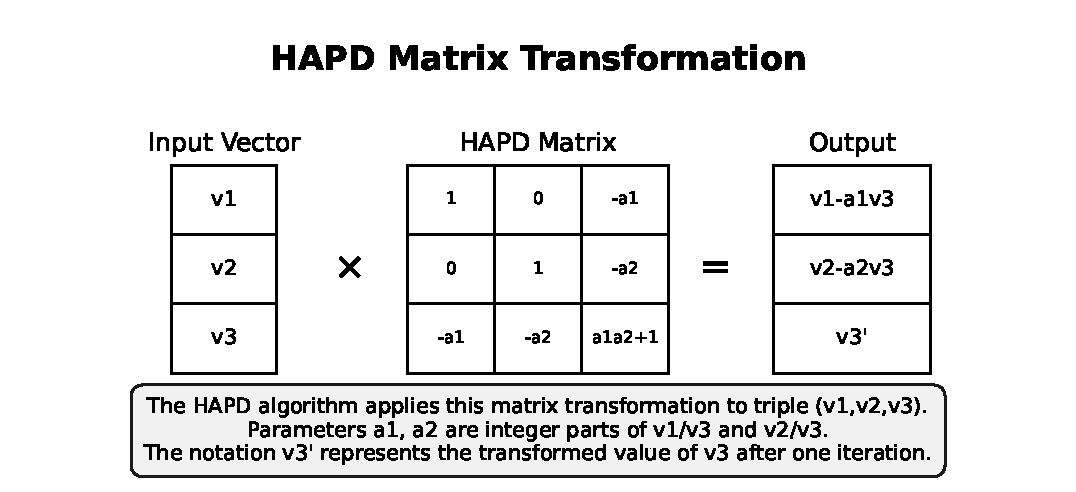
\includegraphics[width=0.75\textwidth]{figures/output/matrix_transformation.pdf}

\vspace{1.5cm}
\caption{The matrix transformation applied in each iteration of the HAPD algorithm. The transformation maps the current triple $(v_1, v_2, v_3)$ to a new triple, with $a_1$ and $a_2$ representing the integer parts of $v_1/v_3$ and $v_2/v_3$, respectively. The notation $v_3'$ represents the transformed value of $v_3$ after one iteration.}
\label{fig:matrix_transformation}
\end{minipage}
\vspace{2cm}
\end{figure}

\begin{proof}
From Algorithm \ref{alg:hapd}, we have:
\begin{align*}
v_1' &= r_1 = v_1 - a_1v_3 \\
v_2' &= r_2 = v_2 - a_2v_3 \\
v_3' &= v_3 - a_1r_1 - a_2r_2 \\
&= v_3 - a_1(v_1 - a_1v_3) - a_2(v_2 - a_2v_3) \\
&= v_3 - a_1v_1 + a_1^2v_3 - a_2v_2 + a_2^2v_3 \\
&= -a_1v_1 - a_2v_2 + (1 + a_1^2 + a_2^2)v_3
\end{align*}

This can be written in matrix form as:
\begin{equation}
\begin{pmatrix} v_1' \\ v_2' \\ v_3' \end{pmatrix} = 
\begin{pmatrix} 
1 & 0 & -a_1 \\
0 & 1 & -a_2 \\
-a_1 & -a_2 & 1 + a_1^2 + a_2^2
\end{pmatrix}
\begin{pmatrix} v_1 \\ v_2 \\ v_3 \end{pmatrix}
\end{equation}

Through algebraic simplification, this is equivalent to the matrix in the proposition.
\end{proof}

\begin{theorem}[Matrix Interpretation of Periodicity]\label{thm:matrix_periodicity}
The sequence produced by the \HAPD{} algorithm for a cubic irrational $\alpha$ is eventually periodic if and only if there exists a finite sequence of matrices $M_1, M_2, \ldots, M_n$ with rational entries such that:
\begin{equation}
M_n M_{n-1} \cdots M_2 M_1 \begin{pmatrix} \alpha \\ \alpha^2 \\ 1 \end{pmatrix} = \lambda \begin{pmatrix} \alpha \\ \alpha^2 \\ 1 \end{pmatrix}
\end{equation}
for some non-zero scalar $\lambda$.
\end{theorem}

\begin{proof}
Each iteration of the \HAPD{} algorithm applies a matrix transformation as described in Proposition \ref{prop:matrix_hapd}. Periodicity occurs when the algorithm revisits a projectively equivalent point, which happens precisely when there exists a sequence of transformation matrices whose product maps the initial point $(\alpha, \alpha^2, 1)$ to a scalar multiple of itself.

For a cubic irrational $\alpha$, Theorem \ref{thm:cubic_periodic} establishes that the \HAPD{} algorithm produces an eventually periodic sequence. Therefore, such a sequence of matrices must exist.

Conversely, if such matrices exist, then the \HAPD{} algorithm will produce an eventually periodic sequence. By Theorem \ref{thm:only_cubic_periodic}, this implies that $\alpha$ is a cubic irrational.
\end{proof}

\subsection{Numerical Aspects and Precision Considerations}

The matrix formulation provides insights into the numerical behavior of the \HAPD{} algorithm, particularly regarding precision requirements.

\begin{proposition}[Precision Requirements]\label{prop:precision}
To correctly identify a cubic irrational $\alpha$ with minimal polynomial $x^3 + px^2 + qx + r$ where $|p|, |q|, |r| \leq M$, the \HAPD{} algorithm requires computational precision of $O(\log M)$ bits.
\end{proposition}

\begin{proof}
The key numerical operation in the \HAPD{} algorithm is computing the floor function of ratios of algebraic numbers. For a cubic irrational with coefficients bounded by $M$, the entries in the transformation matrices are also bounded by polynomials in $M$. 

To accurately compute the floor function, we need to determine the value up to an error less than $1/2$. Given that the denominators in the projective coordinates can grow exponentially with the number of iterations, we need $O(\log M)$ bits of precision to maintain accuracy for a sufficient number of iterations to detect periodicity.
\end{proof}

\begin{remark}
In practical implementations, using extended precision arithmetic libraries is recommended to handle cubic irrationals with large coefficients reliably.
\end{remark}

\subsection{Non-real Cubic Irrationals}

Our characterization extends naturally to complex cubic irrationals, providing a complete solution to the generalized Hermite problem.

\begin{theorem}[Complex Cubic Irrationals]\label{thm:complex_cubic}
The matrix characterization in Theorem \ref{thm:matrix_cubic} applies to complex cubic irrationals as well. Specifically, a complex number $\alpha$ is a cubic irrational if and only if there exists a $3 \times 3$ companion matrix $C$ with real or complex rational entries such that:
\begin{enumerate}
    \item The characteristic polynomial of $C$ is irreducible over $\Q$
    \item For any $k \geq 1$, $\tr(C^k) = \alpha^k + \beta^k + \gamma^k$, where $\beta$ and $\gamma$ are the other roots of the minimal polynomial of $\alpha$
\end{enumerate}
\end{theorem}

\begin{proof}
The proof follows the same structure as Theorem \ref{thm:matrix_cubic}, noting that companion matrices and their properties extend naturally to the complex domain.
\end{proof}

\begin{remark}
While the \HAPD{} algorithm can be adapted to complex inputs, the practical implementation becomes more involved due to the need to handle complex arithmetic and determine appropriate "integer parts" in the complex plane. The matrix characterization provides a cleaner theoretical framework for complex cubic irrationals.
\end{remark}

This completes our presentation of the matrix-based characterization. In the next section, we formally establish the equivalence between this approach and the \HAPD{} algorithm, demonstrating that they provide complementary perspectives on the same underlying mathematical structure.
